\chapter {Design of OGM library}

We should now have all information we need to propose our solution for OGM using C\# language.
Before we start to analyze individual pieces of the library needed for its proper function, we need a list of requirements.

The solution should be able to:
\begin{itemize}
    \item {connect to a database}
    \item {map objects into graph structure}
    \item {map LINQ query into Cypher query}
    \item {execute a command in a database}
    \item {retrieve a result from the database}
    \item {map the result from the database into objects}
\end{itemize}

With these minimal requirements set, we can now go through them, analyze them, and propose individual solutions to them.

\section{Connect to a database}

Neo4j company has created a client for .NET that supports both bolt and neo4j URI schemes. \cite{noauthor_client_nodate} This driver is a standalone NuGet package that is publicly accessible and licensed under Apache 2.0 license. This means we can use this driver in our library as a dependency.

The application should handle the driver's lifecycle. During startup, the application should create an instance of the driver and then correctly destroy this instance on exit. The lifecycle will be managed by our library or by using DIC.

Before we create an instance of the driver, we need to pass the correct configuration for the driver. Configuration for the driver and session must be created and maintained. .NET does contain a configuration manager used with the linkage to dependency injection.

Here is visualisation of connections between components:

\begin{figure}[H]
    \centering
    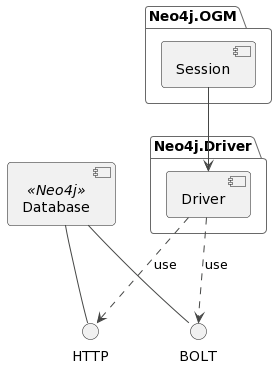
\includegraphics[width=0.4\textwidth]{content/components.png}
    \caption{Components diagram}
\end{figure}

\subsection{Conclusion}

We will use Neo4j's official driver for connection, but we need to encapsulate it into our library. This means we need to create a configuration structure and configuration builder, which will then be used to connect to the database.

\section {Map objects into graph structure}

If we want to translate queries from the object paradigm into Cypher correctly, we need to know the graph structure described in our domain.

What we are trying to do is create metadata. To build metadata, we first need information, which assemblies contain models representing nodes and relationships in a graph. A developer must declare these assemblies as it is necessary to limit the scope that will be scanned using reflection.

Solutions that we analyzed in the previous chapter are internally working very similarly. Both are scanning assemblies or packages on initialization (Java uses packages vs. C\# uses assemblies/namespaces), and we will borrow some of the features from these solutions into ours.
Developers of our library will need to define a set of assemblies. During the initialization of our library, we will scan these assemblies and create a metadata object with information about the user-defined graph.

\subsection {Annotations}

To create a metadata object, we need to identify and process nodes and relationships. We need to have a way for developers to describe each node and its relationship with all properties they would want to define, and which we also need to build the metadata object correctly.

We already have a solution to this problem, and Neo4j also uses it to solve the same issue. We will use annotations using attributes. Using these annotations, we can describe nodes and their relationships.

We will look for these annotations during initialization using reflection, which is well supported by C\# and .NET. With annotation, we can describe the graph and create the metadata object.

\subsection {Entity mapper}

Entity mapper should be able to map entities into statements that could then be translated into Cypher query. It should be able to use generated metadata correctly
to map both nodes and relationships.

For this purpose, we will define a interface \texttt{IEntityMapper}. This interface will contain
this list of public methods:

\begin{itemize}
    \item {\texttt{Map}: this method map an entity to a \texttt{ICompilerContext}}
    \item {\texttt{CompilerContext}: this method returns a current instance of \texttt{ICompilerContext}}
\end{itemize}

In the picture \ref{fig:IEntityMapperClassDiagram} is class diagram with interfaces and also classes that implements these interfaces.
The interface \texttt{ICompilerContext} contains methods for controling context of mapped nodes and relationships. These methods
are used during mapping an entity in \texttt{IEntityMapper.Map} method to map an entity for Cypher query.

\begin{figure}[H]
    \centering
    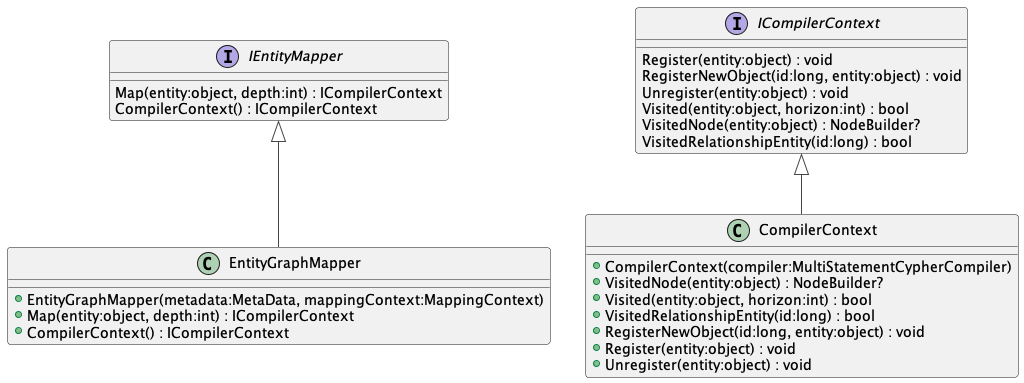
\includegraphics[width=0.8\textwidth]{content/entitymapper.png}
    \caption{\texttt{IEntityMapper} and \texttt{ICompilerContext} class diagrams}
    \label{fig:IEntityMapperClassDiagram}
\end{figure}

\section {Map LINQ query into Cypher query}

We can connect to a database, and we also have mapped the whole graph and created metadata to navigate through schema. Now, we need the ability to translate a query written in LINQ to a query in Cypher.

We need to use a similar approach to mimic how Entity Framework Core translates a LINQ query to SQL. If we want them to be translated correctly,
we need to define our encapsulation for nodes and relationships with properties. This encapsulation will be similar to DbSet found in Entity Framework.

Our \texttt{DbSet} class will also implements interface \texttt{IQueryable<T>}. In our case, the DbSet class will be created by \texttt{ISession}.



\todo[inline]{Summary}
